This chapter outlines the methodology employed to achieve the project objective. Firstly, a suitable quarter-car model for the active suspension system is selected. Subsequently, a mathematical model is derived, followed by its representation in state-space form. Controllability analysis is then performed on the system. Based on these findings, the following chapter delves into the implementation and evaluation of various control strategies designed to enhance the performance of the active suspension system.

\section{Two-DOF Quarter Car Model}
To analyze the parameters related to the suspension system, a simplified quarter-car model, as shown in \ref{fig:m1}(a), was utilized. The quarter-car model was chosen due to its simplicity and common use in analyzing the vertical vibrations caused by railway disturbances in vehicle dynamic models.

The vehicle's mass is divided into two: the sprung mass (representing the vehicle body) and the unsprung mass (tire). Suspension springs and dampers connect the sprung and unsprung masses and the road.

Both the transverse and longitudinal deflections are considered insignificant compared to the vertical deflections of the suspension system. For the passive suspension system is shown in \ref{fig:m1}(b).

\begin{figure}[H]
	\centering
	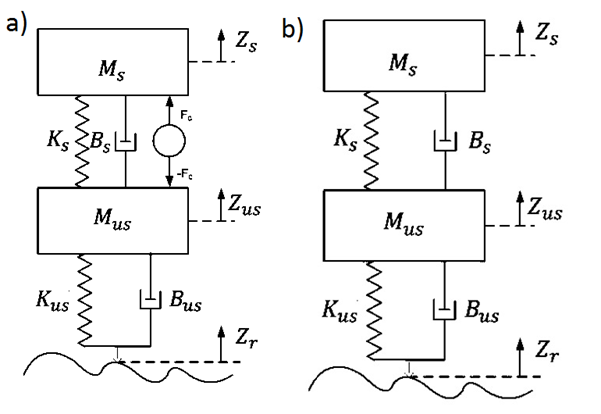
\includegraphics[width=0.4\linewidth]{model1.png}
	\caption{Active suspension system (a) and Passive suspension (b).}
	\label{fig:m1}\cite{lqr_acti}
\end{figure}

\begin{table}[H]
	\centering
	\caption{Parameters of Quarter Car Model.}
	\begin{tabular}{l|l}
		\hline
		$M_s$ & Vehicle body mass or sprung mass. \\
		$M_{us}$ & Unsprung mass (Tire, wheel, brake caliper, suspension links, etc.) \\
		$K_s$ & Spring constant for the sprung mass. \\
		$K_{us}$ & Spring constant for the unsprung mass. \\
		$B_s$ & Inherent damping coefficient for the suspension system. \\
		$B_{us}$ & Inherent damping coefficient for vehicle wheel assembly. \\
		$F_c$ & The active suspensions actuator control force. \\
		$Z_s$ & Vehicle (sprung mass) body displacement. \\
		$Z_{us}$ & Vehicles wheel displacement and the unsprung masses displacement \\
		$Z_r$ & Excitation due to the railway disturbance. \\
		\hline
	\end{tabular}
	\label{table:qcm_image}
\end{table}

\newpage
\subsection{Passive Suspension Model}
The parameters for the PSS are given in the following table:

\begin{table}[h]
	\centering
	\caption{Passive Model Parameters}
	\begin{tabular}{lccc}
		
		\hline
		\textbf{Parameter} & \textbf{Symbol} & \textbf{Value}  & \textbf{Unit}  \\
		\hline
		
		Sprung mass & \( M\)& 30 & kg\\
		Unsprung mass & \( m \)& 13 & kg\\
		Spring stiffness & \( k \)& 6921 & N/m\\ 
		Tire stiffness & \( k_{t} \)& 81000 & N/m\\
		Damper average damping coefficient & \( b_{s} \)& 900 & N s/m\\
		Tire damping coefficient & \( b_{tr} \)& 0 & N s/m\\
		
		\hline
		\label{table:Parameter}
	\end{tabular}
\end{table}
\begin{figure}[H]
	\centering
	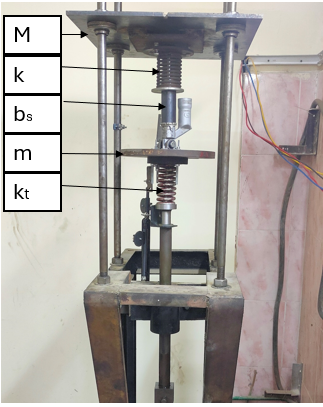
\includegraphics[width=0.45\textwidth]{layout labeled.png}
	\caption{PSS Physical Model, by Ain Shams Univresity Students as Graduation Project, Fall 2024, Automotive Department.}
	\label{fig:Passive layout}
\end{figure}

\newpage
\subsection{Active Suspension Model}
The parameters of the modified system is listed in the table below.

\begin{table}[h]
	\centering
	\caption{Active Model Parameters}
	\begin{tabular}{lccc}
		
		\hline
		\textbf{Parameter} & \textbf{Symbol} & \textbf{Value}  & \textbf{Unit}  \\
		\hline
		
		Sprung mass & \( M \)& 34 & kg\\
		Unsprung mass & \( m \)& 11 & kg\\
		Spring stiffness & \( k \)& 6921 & N/m\\ 
		Tire stiffness & \( k_{t} \)& 81000 & N/m\\
		\hline
		\label{table:Parameter}
	\end{tabular}
\end{table}

The setup of the modified Active suspension System is shown in the following figure:

\begin{figure}[H]
	\centering
	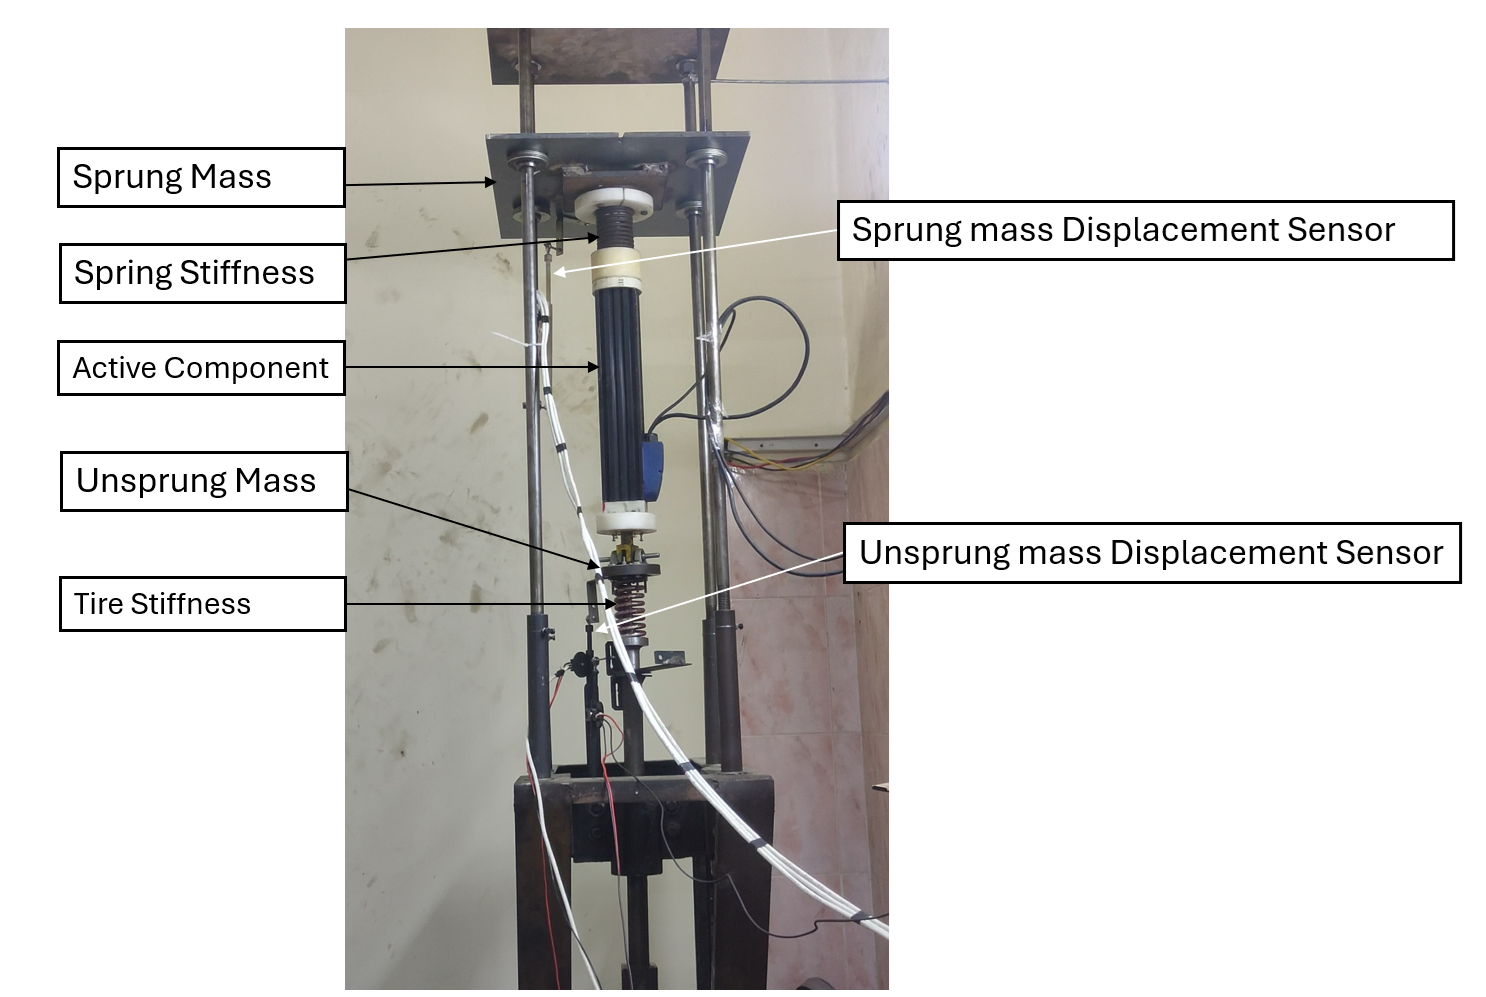
\includegraphics[width=0.9\textwidth]{Active Setup.png}
	\caption{ASS Physical Model, by Ain Shams Univresity Students as Graduation Project, Spring 2024, Automotive Department.}
	\label{fig:Active schematic diagram}	
\end{figure}


\newpage
\subsection{Equation Of Motion}

\textbf{Sprung Mass}
\begin{equation}
M_s\ddot{Z}_s = B_s\dot{Z}_{us} - B_s\dot{Z}_s - K_s(Z_s - Z_{us}) + F_c
\end{equation}

\begin{equation}
\ddot{Z}_s = \frac{B_s\dot{Z}_{us}}{M_s} - \frac{B_s\dot{Z}_s}{M_s} - \frac{K_s(Z_s - Z_{us})}{M_s} + \frac{1}{M_s}F_c
\end{equation}

\textbf{Unsprung Mass}
\begin{equation}
M_{us}\ddot{Z}_{us} = -B_s\dot{Z}_{us} - B_{us}\dot{Z}_{us} + B_s\dot{Z}_s + B_{us}\dot{Z}_r - K_s(Z_{us} - Z_s) - K_{us}(Z_{us} - Z_r) - F_c
\end{equation}\\


\begin{equation}
\ddot{Z}_{us} = -\frac{B_s\dot{Z}_{us}}{M_{us}} - \frac{B_{us}\dot{Z}_{us}}{M_{us}} + \frac{B_s\dot{Z}_s}{M_{us}} + \frac{B_{us}\dot{Z}_r}{M_{us}} - \frac{K_s(Z_{us} - Z_s)}{M_{us}} - \frac{K_{us}(Z_{us} - Z_r)}{M_{us}} - \frac{1}{M_{us}}F_c
\end{equation}\\

\subsection{State Space Model}
A state-space representation is a mathematical model used in modern control theory and system analysis to describe the behavior of a dynamic system. It offers a concise and systematic approach to representing the evolution of a system over time. In contrast to the frequency-domain representation (e.g., transfer functions), which characterizes a system's input-output relationship in terms of frequencies, the state-space representation provides a time-domain description.\\

\textbf{The general state-space representation is given by the following:}
$$\dot{x}_{(t)}=Ax_{(t)}+Bu_{(t)}$$
$$y_{(t)}=Cx_{(t)}+Du_{(t)}$$

\begin{itemize}
	\item $x$: State variables vector.
	\item $\dot{x}$: Represents the time derivative of the state variables vector.
	\item $y$: Output vector.
	\item $u$: Input vector.
	\item $A$: System matrix.
	\item $B$: Input matrix.
	\item $C$: Output matrix.
	\item $D$: Feedforward matrix.\\
\end{itemize}


\begin{table}[h!] % You can adjust the placement options (h!, t, b, p)
	\centering
	\caption{State Variables} 
	\begin{tabular}{|c|c|}
		\hline
		\textbf{Variable} & \textbf{Description} \\ \hline
		$X_1 = Z_s - Z_{us}$ & suspension travel \\ \hline
		$X_2 = \dot{Z}_s$ & sprung mass velocity \\ \hline
		$X_3 = Z_{us} - Z_r$ & wheel deflection \\ \hline
		$X_4 = \dot{Z}_{us}$ & wheel vertical velocity \\ \hline
	\end{tabular}
\end{table}



\newpage
\textbf{Inputs:} We will consider the input $\boldsymbol{u}$ into the system as the road disturbance velocity $\dot{Z}_r$ and the actuator input $F_c$.\\

\textbf{Outputs:} We will consider outputs $\boldsymbol{y}$ from the system as the suspension travel $Z_s-Z_{us}$ and the vehicle body (sprung mass) acceleration $\ddot{Z}_s$.\\

Using the above equations of motion, the state-space model of the active suspension system can easily be obtained and be written in the matrix form shown below:

\begin{equation}
\begin{bmatrix}
	\dot{x}_1 \\
	\dot{x}_2 \\
	\dot{x}_3 \\
	\dot{x}_4
\end{bmatrix} = 
\begin{bmatrix}
	0 & 1 & 0 & -1 \\
	-\frac{K_s}{M_s} & -\frac{B_s}{M_s} & 0 & \frac{B_s}{M_s} \\
	0 & 0 & 0 & 1 \\
	\frac{K_s}{M_{us}} & \frac{B_s}{M_{us}} & -\frac{K_{us}}{M_{us}} & -\frac{B_s + B_{us}}{M_{us}} 
\end{bmatrix}
\begin{bmatrix}
	x_1 \\
	x_2 \\
	x_3 \\
	x_4
\end{bmatrix} + 
\begin{bmatrix}
	0 & 0 \\
	0 & \frac{1}{M_{s}} \\
	-1 & 0 \\
	\frac{B_{us}}{M_{us}} & -\frac{1}{M_{us}} \\
\end{bmatrix}
\begin{bmatrix}
	\dot{Z}_r \\
	F_c
\end{bmatrix}
\end{equation}


\begin{equation}
\begin{bmatrix}
	Y_1 \\
	Y_2
\end{bmatrix} = 
\begin{bmatrix}
	1 & 0 & 0 & 0 \\
	-\frac{K_s}{M_s} & -\frac{B_s}{M_s} & 0 & \frac{B_s}{M_s} 
\end{bmatrix}
\begin{bmatrix}
	X_1 \\
	X_2 \\
	X_3 \\
	X_4
\end{bmatrix} + 
\begin{bmatrix}
	0 & 0 \\
	0 & \frac{1}{M_s}
\end{bmatrix}
\begin{bmatrix}
	\dot{Z}_r \\
	F_c
\end{bmatrix}
\end{equation}







\section{State Space Controllability}
State-space controllability refers to the ability to drive a system from any initial state to any desired state within a finite time using an appropriate control input. A linear time-invariant (LTI) system represented in state-space form, is controllable if the controllability matrix has full rank. When this condition is met, it ensures that the system's states can be influenced by the control input, enabling effective feedback control design.\newline

$\mathcal{C} = \left[ \begin{matrix}
	B & AB & A^2B & \cdots & A^{n-1}B
\end{matrix} \right]$\newline

$rank(\mathcal{C}) = n$


\begin{verbatim}
	% MATLAB script
	ms  = 34;           % Sprung Mass (kg)
	mus = 11;           % Unsprung Mass (kg)
	ks  = 6921;         % Suspension Stiffness (N/m)
	kus = 81000;        % Wheel stiffness (N/m)
	bs  = 0;            % Suspension Inherent Damping coefficient (sec/m)
	bus = 0;            % Wheel Inhenrent Damping coefficient (sec/m)
	
	%% System Dynamics for the Active Suspension system.
	A = [ 0 1 0 -1 ;
	-ks/ms -bs/ms 0 bs/ms;
	0 0 0 1; 
	ks/mus bs/mus -kus/mus -(bs+bus)/mus];
	
	B = [0  0 ; 
	0 1/ms ; 
	-1  0 ;
	bus/mus -1/mus ];
	
	C = [ 1 0 0 0 ; 
	-ks/ms -bs/ms 0 bs/ms ];
	
	D = [0 0;
	0 0;
	0 0;
	0 0;
	0 0;
	0 1/ms];
	
	%% Controllability
	rank(ctrb(A,B))
\end{verbatim}

The following figure shows that the system is controllable, because its controllability matrix is full rank which is equal to the number of states.\newline

\begin{figure}[H]
	\centering
	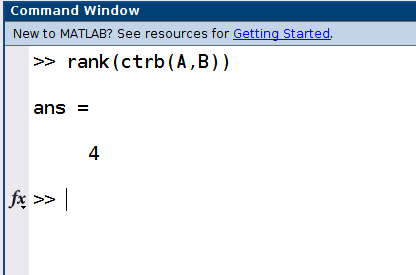
\includegraphics[width=0.4\textwidth]{ctrb.png}
	\caption{Conrollability matrix is full rank}
	\label{fig:ctrb}	
\end{figure}


\section{Road Disturbance Profile}
The slider-crank mechanism as shown in\ref{fig:sliderr} is used to simulate road. This mechanism converts the rotational motion of a crank into the linear motion of a slider, effectively replicating the vertical displacement experienced by a vehicle's suspension system when driving over uneven road surfaces which can change road amplitude by changing eccentricity from crank disk.
\begin{figure}[H]
	\centering
	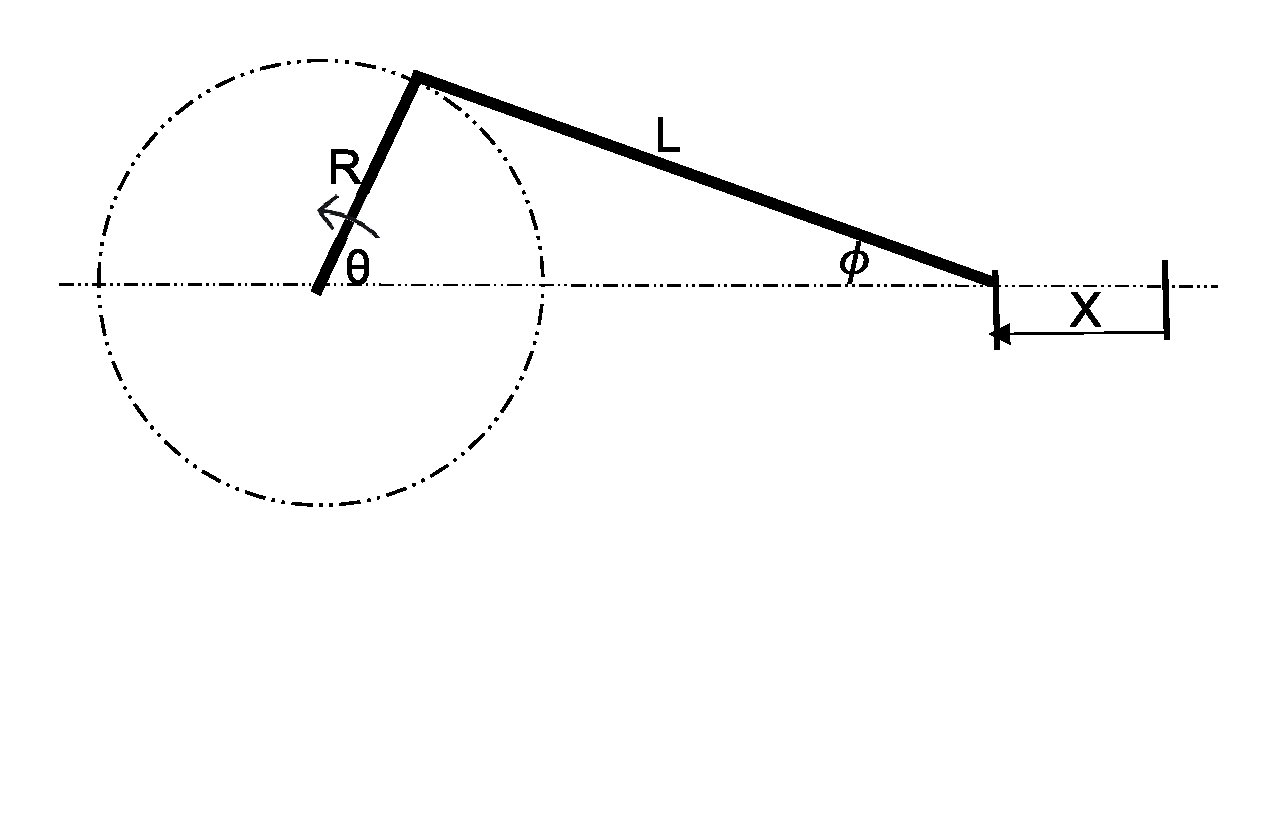
\includegraphics[trim=0cm 4cm 0cm 0cm, clip, width=1\linewidth]{sliderr.pdf}
	\caption{the slider crank mechanism}
	\label{fig:sliderr}
\end{figure}

\begin{itemize}
	\item $R$: Length of the crank
	\item $L$: Length of the connecting rod
	\item $\theta $: Angle of the crank 
	\item $x$: Position of the slider
\end{itemize}
\newpage
\subsection*{Kinematic Equations}

The position \( x \) of the slider can be determined using the crank angle \( \theta \) and \( \phi \) be the angle of the connecting rod with the horizontal. The position \( x \) of the slider can be expressed as:


\begin{equation}
	x = R \left[ 1 - \cos \theta + n - \sqrt{n^2 - \sin^2 \theta} \right] 
\end{equation}

since \( n = \frac{L}{R} \).